\section{Anwendungsentwicklung}
\label{sec:anwendungeentwicklung}

\paragraph{Client-Server-Architektur}
\begin{figure}[H]\centering\label{ClientServer}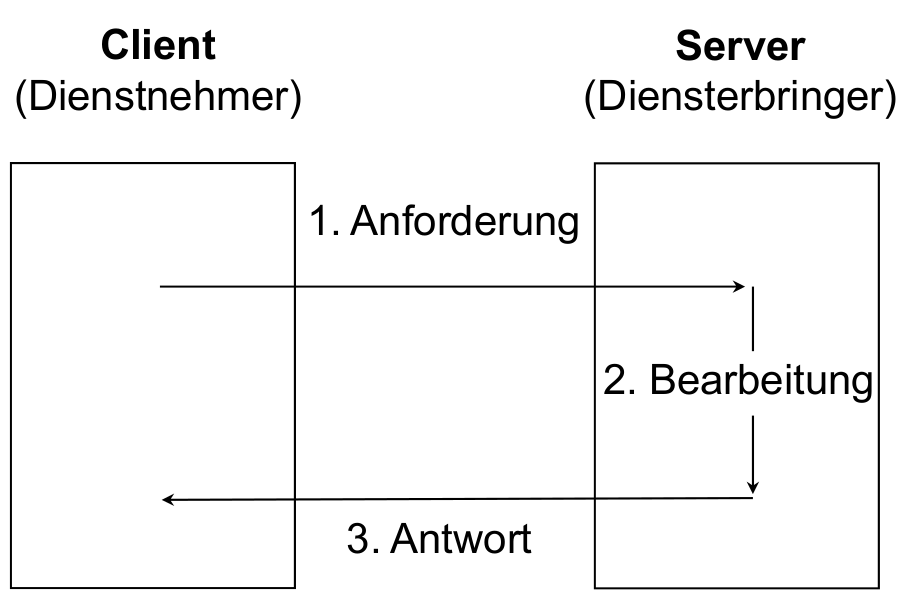
\includegraphics[width=0.25\textwidth]{ClientServer}\end{figure}
\begin{items}
	\item Erfordert \\*
		- Kenntnis über angebotene Dienste \\*
		- Protokoll zur Regelung der Interaktion
\end{items}

\paragraph{Zwei Schichten-Architektur}
\begin{figure}[H]\centering\label{ZweiSchichtenArchitektur}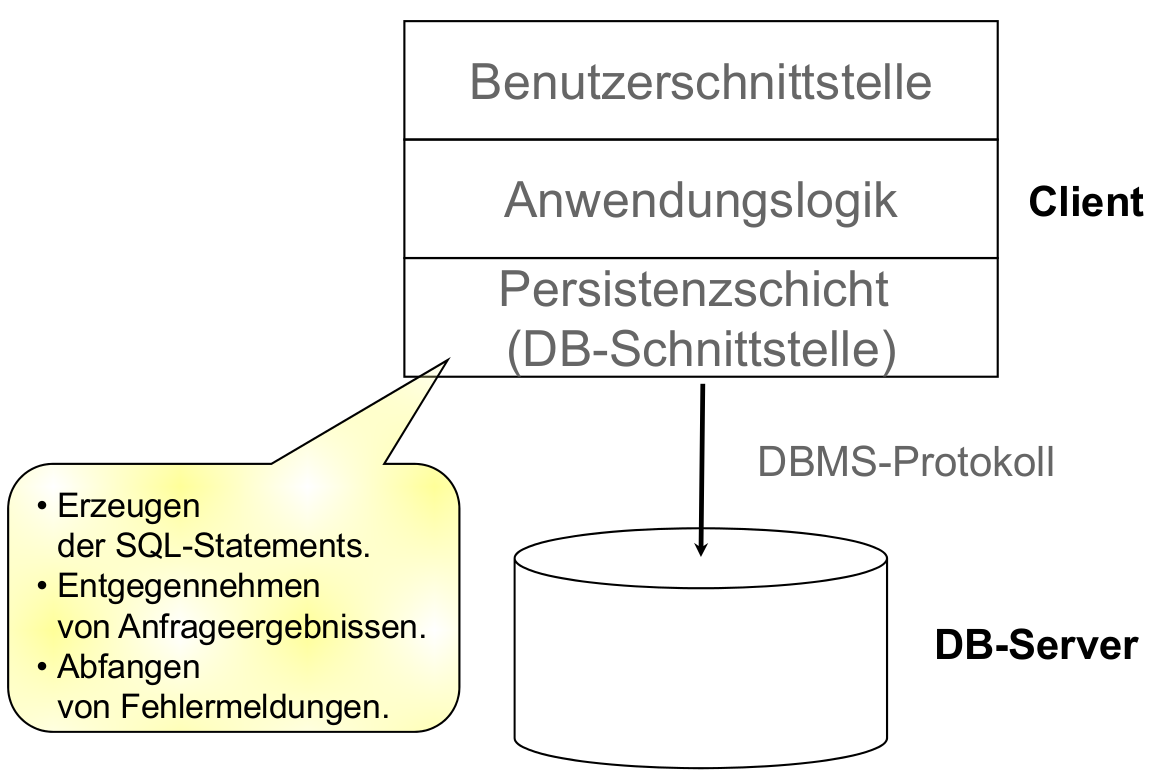
\includegraphics[width=0.33\textwidth]{ZweiSchichtenArchitektur}\end{figure}

\paragraph{Drei Schichten-Architektur}
\begin{figure}[H]\centering\label{DreiSchichtenArchitektur}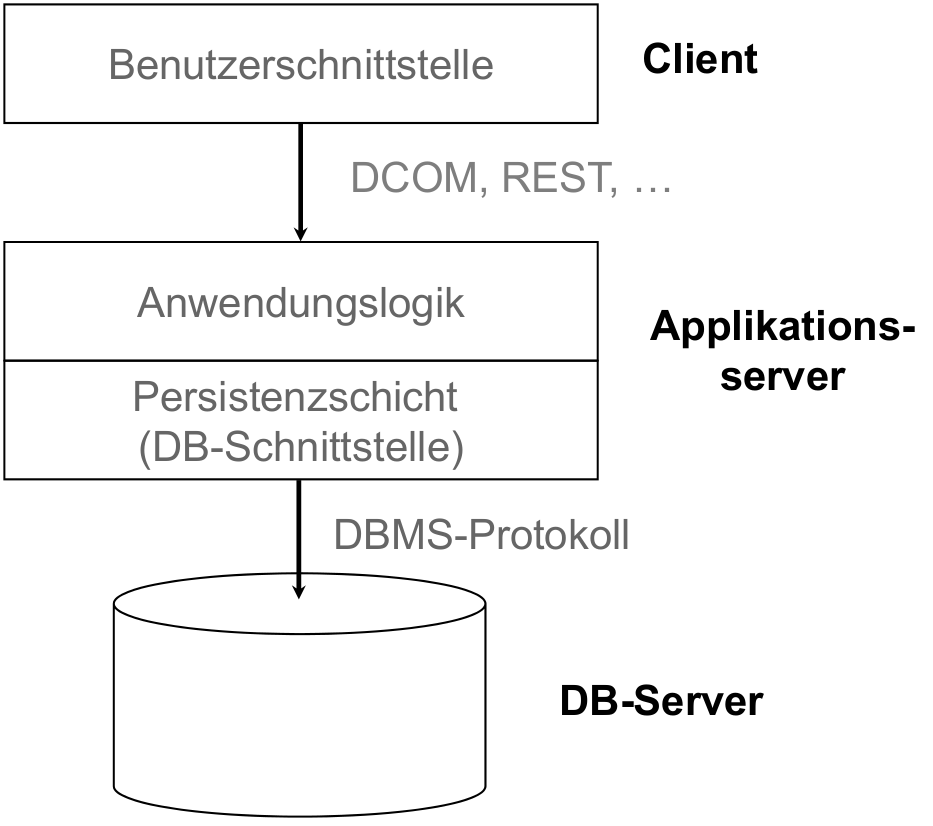
\includegraphics[width=0.33\textwidth]{DreiSchichtenArchitektur}\end{figure}

\paragraph{Anwendungslogik}
\begin{items}
	\item \textbf{Anwendungslogik}: Algorithmen, die anwendungsspezifisches Wissen beinhalten
	\item Personal-DB entählt Mitarbeiter-Daten
		\\*
		\( \leadsto \) Anwendung: schlägt Teamleiter für konkrete Projekte vor
		\\*
		\( \leadsto \) Bedeutsamkeit der Fähigkeiten usw. Anwendungsteil
\end{items}

\paragraph{Cursor-Konzept}
\begin{items}
	\item Cursor \( \equiv \) Iterator
	\item Programmiersprachen: einzelne Datenobjekte als zugrundeliegende Struktur
\end{items}



\paragraph{Programmiersprachenanbindung}
\begin{figure}[H]\centering\label{Programmiersprachenanbindung}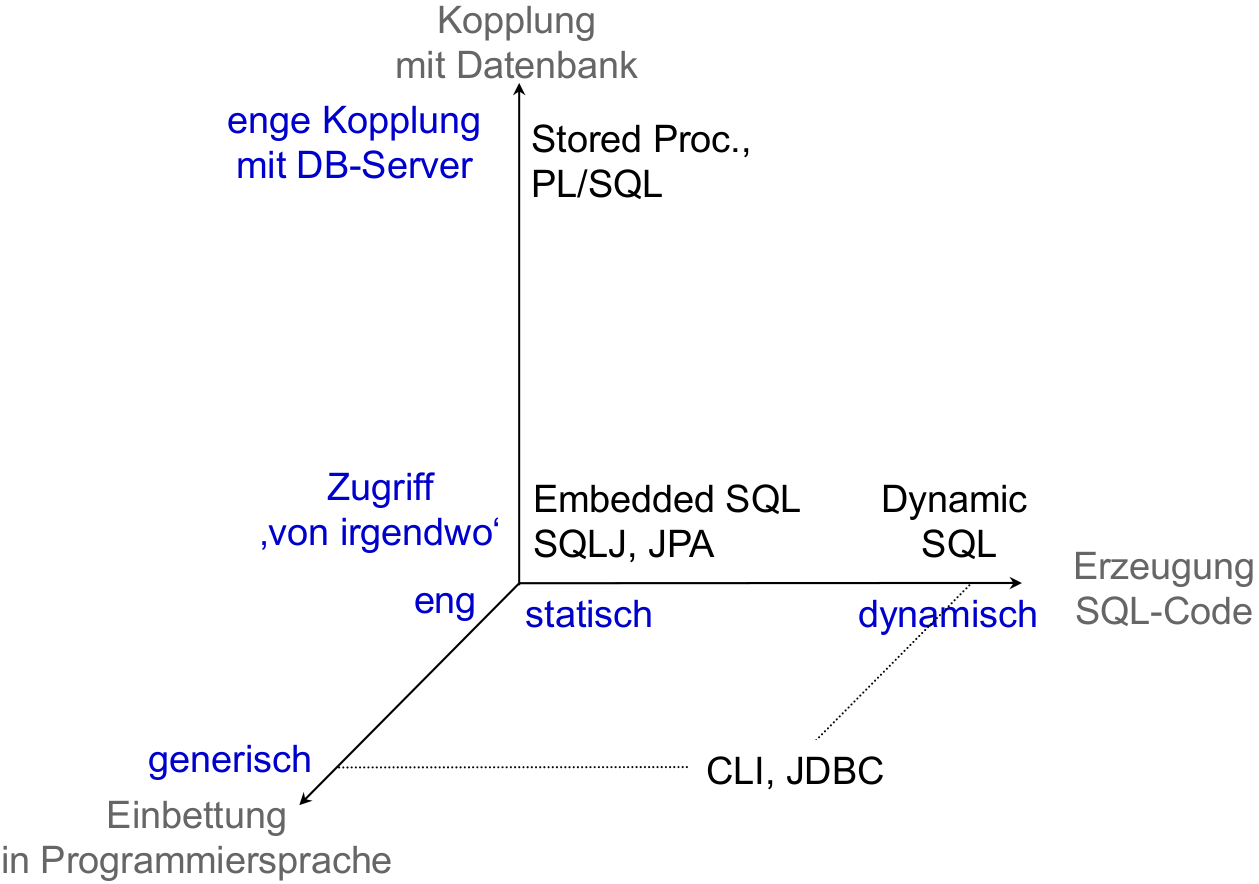
\includegraphics[width=0.33\textwidth]{Programmiersprachenanbindung}\end{figure}

\paragraph{Prepared Statements}
\begin{items}
	\item Reduzieren Ausführungszeit, da bereits vorab kompiliert
	\item
		\begin{lstlisting}[language=java,showstringspaces=false]
PreparedStatement updateSales = 
  con.prepareStatement('UPDATE COFFEES 
  SET SALES = ? WHERE COF_NAME LIKE ?');
		\end{lstlisting}
	\item \lstinline[language=java]{upcdateSales.setInt(1,75);}
\end{items}

\paragraph{Gespeicherte Prozeduren}
\begin{items}
	\item In DB-Server verwaltete und ausgeführte Software-Module in Form von Prozeduren/Funktionen
	\item Aufruf aus Anwendungen/Anfragen heraus
	\item \( \leadsto \) Weniger Kontextwechsel in Anwendung
\end{items}

\paragraph{Variablen und Typen}
\begin{items}
	\item \lstinline[language=sql]{DECLARE preis NUMBER;}
	\item Stellt sicher, dass Attributtyp in DB identisch zu Typ in Programm ist
\end{items}

\paragraph{Kontrollfluss}
\begin{items}
	\item
	\begin{lstlisting}[language=sql]
DECLARE
  a NUMBER;
  b NUMBER;
BEGIN
  SELECT e,f INTO a,b
  FROM T1 WHERE e>1;
  IF b=1 THEN
    INSERT INTO T1 VALUES(b,a);
  ELSE
    INSERT INTO T1 VALUES(b+10,a+10);
  END IF;
END;
.
run;
	\end{lstlisting}
\end{items}

\paragraph{Performance Anti-Patterns}
\begin{items}
	\item \textbf{Excessive Dynamic Allocation}:
		\\*
		Häufige unnötige Objekterstellung/-zerstörung derselben Klasse
	\item \textbf{The Stifle}:
		\\*
		Unpassende DB-Schnittstellennutzung
	\item \textbf{Circuitous Treasure Hunt}:
		\\*
		Abfrage von Relation A, damit Relation B abfragen,\dots
	\item \textbf{Sisyphus DB Retrieval}:
		\\*
		Riesige Datenmenge abfragen, obwohl nur wenige Einträge nötig
	\item \textbf{Spaghetti Query}:
		\\*
		Mehrere Informationsbedürfnisse in einer Anfrage
	\item \textbf{Insufficient Caching}:
		\\*
		Zu wenig Caching
	\item \textbf{Wrong Caching Strategy}:
		\\*
		Falsche Objekte werden in Cache abgelegt
\end{items}

\begin{fragen}
	\item Erläutern Sie die Dimensionen des Raums der Möglichkeiten des Zugriffs auf Datenbanken aus Anwendungen heraus.
	\item Erläutern Sie die Begriffe \\*
		- Anwendungslogik, \\*
		- Cursor, \\*
		- Call-Level Interface, \\*
		- Host-Variablen.
	\item Kann man mit Embedded SQL sicherstellen, dass keine Schema-spezifischen Fehler auftreten? Wenn ja, wie geht es?
	\item Was sind die Vorteile von Stored Procedures? Erläutern Sie das Konzept.
\end{fragen}